Spočítejte
\begin{enumerate}

	\item primitivní funkci $\int \sin(x) \dx$,

		\solution{
			Primitivní funkce k $\sin(x)$ je $-\cos(x) +C$.
		}

	\item určitý integrál $\int_0^\pi \sin(x) \dx$,

		\solution{
			Využijeme definice Newtonova integrálu, která říká, že pokud $F$ je na $[a, b]$ primitivní funkce k $f$, pak
			$$\int_a^b f(x) \dx = [F(x)]_{a}^{b} = F(b) - F(a)$$

			\begin{align*}
				\int_0^\pi \sin(x) \dx &= [-\cos(x) + C]_0^\pi \\
				&= ((-\cos(\pi) + C) - (-\cos(0) + C)) \\
				&= -\cos(\pi) - (-\cos(0)) \\
				&= 2
			\end{align*}

			Geometrický význam vidíme na Obrázku~\ref{fig:sin_0_pi}.
			\begin{figure}[H]
				\centering
				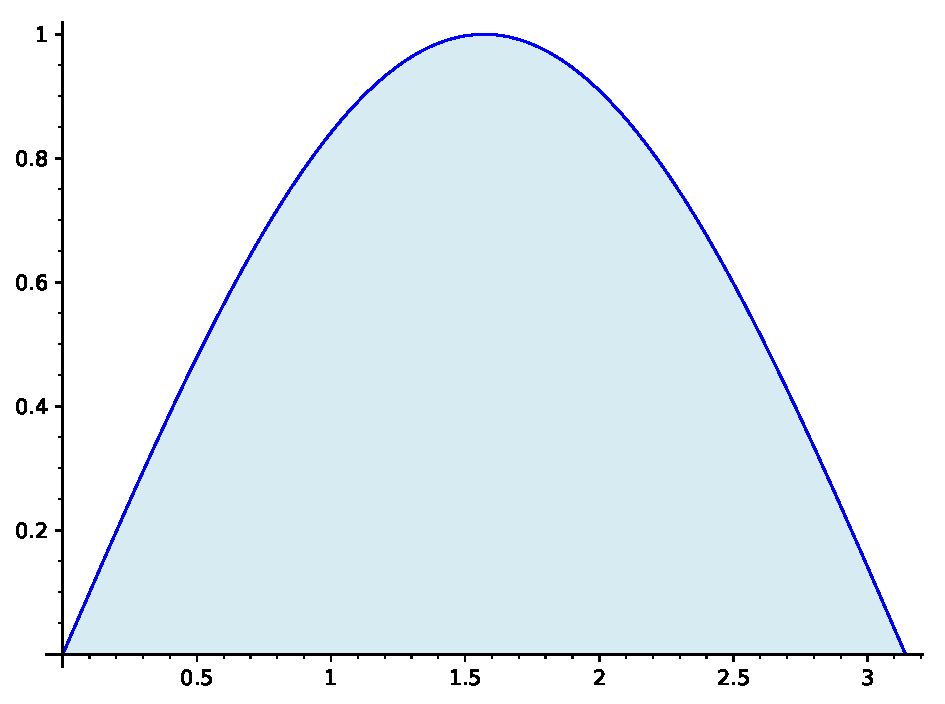
\includegraphics{cviceni_13/fig/sin_0_pi.pdf}
				\caption{$\int_0^\pi \sin(x) \dx = 2$}
				\label{fig:sin_0_pi}
			\end{figure}
		}

	\item určitý integrál $\int_0^{2\pi} \sin x \dx$.

		\solution{
			Obdobně:
			$$\int_0^{2\pi} \sin x \dx = -[\cos x]_0^{2\pi} = -(\cos(2\pi) - \cos 0) = -(1-1) = 0 $$

			Geometrický význam vidíme na Obrázku~\ref{fig:sin_0_2pi}.
			\begin{figure}[H]
				\centering
				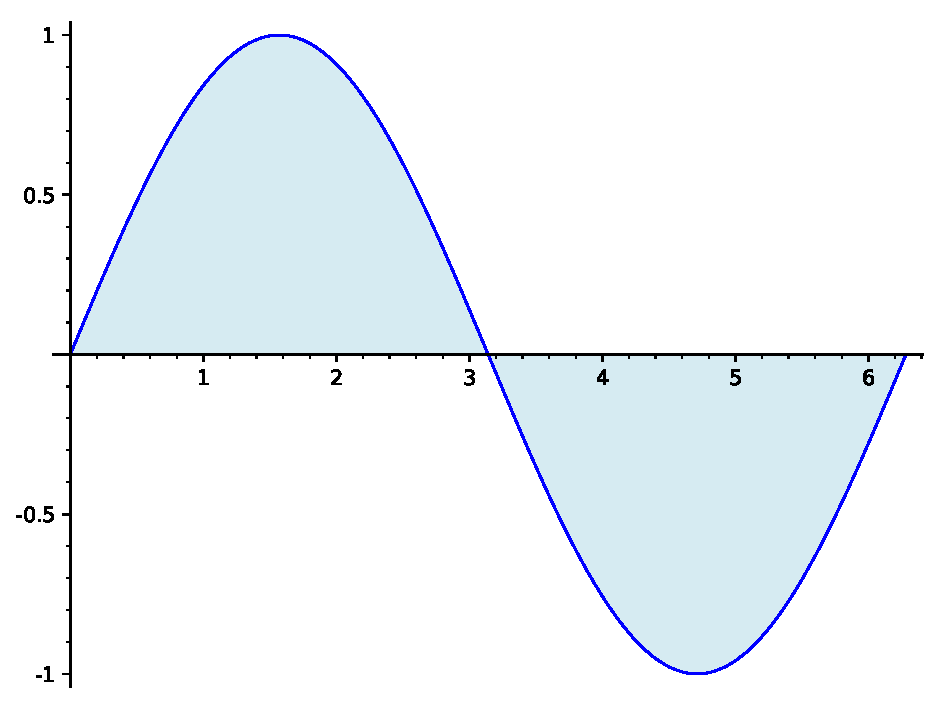
\includegraphics{cviceni_13/fig/sin_0_2pi.pdf}
				\caption{$\int_0^{2\pi} \sin(x) \dx = 2 - 2 = 0$}
				\label{fig:sin_0_2pi}
			\end{figure}
		}
		
\end{enumerate}

